\chapter{Planning}
Before any design or work could be done, an appropriate method of organisation had to be chosen:

\section{Waterfall}
Waterfall (and similar) project management styles are linear, stage based development. Each tier of development (as shown in diagram \ref{fig:waterfall}) must be completed before advancing to the next. This approach helps determines issues that could occur later and usually results in better documentation. However, any issue or requirement change requires reverting back to a previous tier \citep{agilevswaterfall}.

\begin{figure}[H]
    \centering
    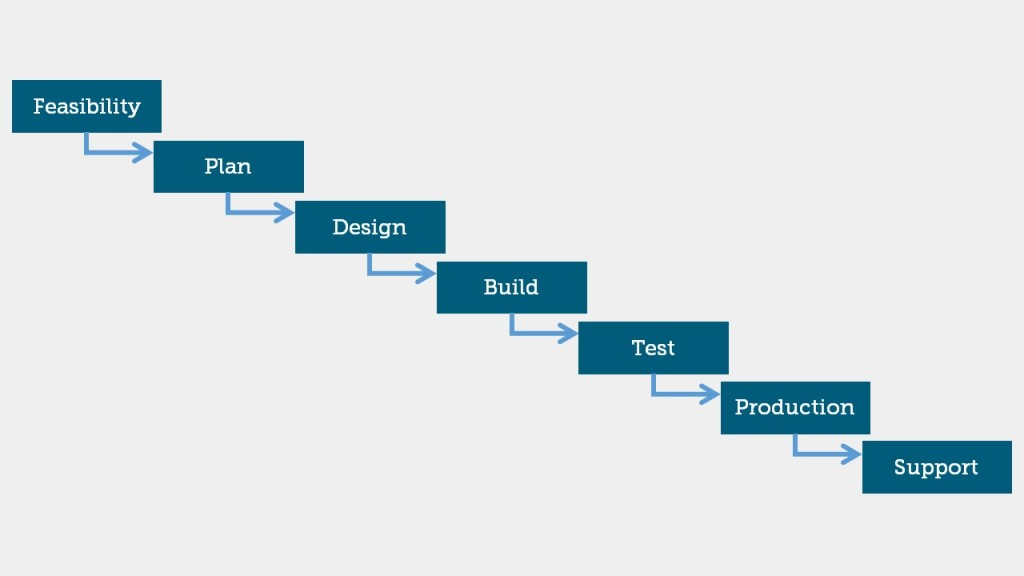
\includegraphics[width=0.8\textwidth]{figs/3/waterfall}
    \caption{Waterfall Stages \citep{agilevswaterfall}}
    \label{fig:waterfall}
\end{figure}

\section{Agile}
Conversely, agile development is a process of continuous, incremental delivery. Each iteration of work is planned briefly and implemented whilst a backlog of work is maintained, allowing for cross functional teams that focus on regular contact with a client leading to short feedback cycles. This ensures that a solution is developed to closer to the customers (often changing) requirements.

\begin{figure}[H]
    \centering
    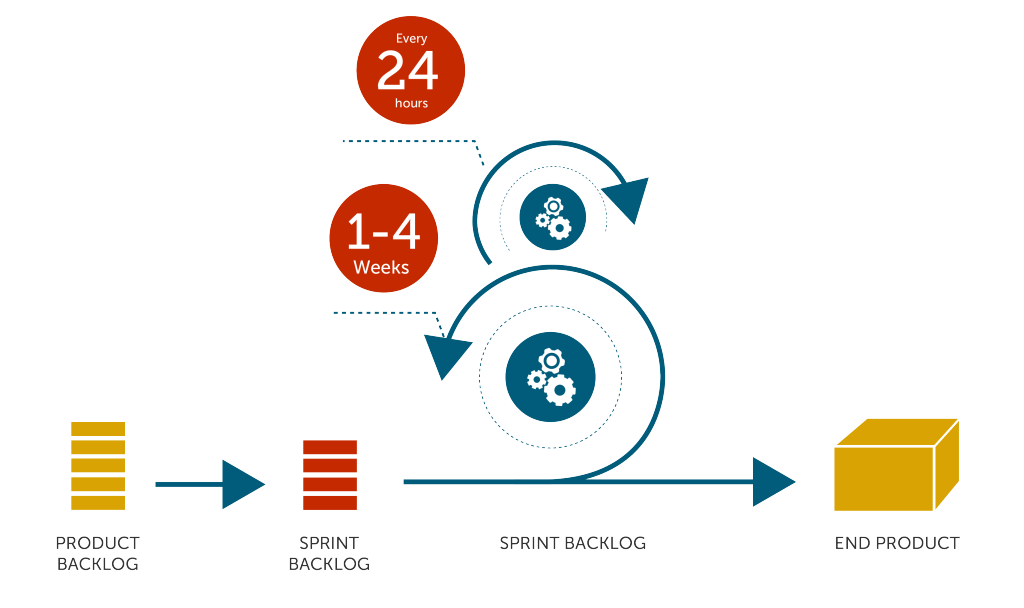
\includegraphics[width=0.8\textwidth]{figs/3/agile}
    \caption{Agile Cycle \citep{agilevswaterfall}}
    \label{fig:agile}
\end{figure}

\section{Outcome: SCRUM}
The agile approach was chosen however agile is an abstract idea. Figure \ref{fig:agile} shows a concrete method of applying the agile methodology to a project. Every iteration (called a `sprint') in scrum lasts one to four weeks and every day the team meet for `stand ups'.


\section{Team Dynamics}
\subsection{Meetings}
As an agile team there would be at least three contact hours a day, every working day. These meetings would be identical to a working day at an agile software development firm. The first hour would often consist of development, followed by a stand up where each team member would update each other on the previous days success and failings and what tasks were to be completed before the next meeting. These `stand-ups' would last no more than 10 minutes. This allowed the team to stay up-to-date with the state of the product. Development would continue afterwards and for 2 hours alone. 

Every week there was a meeting with the project supervisor, where they were updated of the weeks progress and any design changes. These meetings were key to extending our research as the project supervisor had a wealth of knowledge on the subject. Until the third deliverable, the client joined these meetings. This would allow the regular feedback cycles required of SCRUM. Also, by keeping the client up to date, they could steer development. Allowing the project to be built towards the next criteria she desired.

\subsection{Communication}
SCRUM ensured the project was well managed however a key aspect of agile is person to person interaction, not only with the customer but within the team as well (criteria 6 in the agile manifesto \cite{agile:manifesto}). By applying eXtreme Programming (XP) values \citep{XP:values}, this ensured that criteria was fulfilled. 

Respect and communication were key when working in conjunction with SCRUM. A mantra naturally formed ``The work for the team was more important than an individual's''. When a person was stuck on a bug, more team members would help fix it. This close contact also allowed for impromptu design meetings whenever necessary. 

\subsection{Retrospectives}
At the end of each iteration we completed a `retrospective'. This helped us discuss any successes or failures over the previous weeks. It ensured that everyone had a voice and a place to be heard without distraction. This helped us look at the efficiency of our agile process and tailor it to our needs.

In the figure \ref{fig:retro}, you can see the starfish approach was taken. There are five categories, in black, where items are placed that the team should keep doing; do more of; start doing; stop doing and do less of. The team then went through the sections explained what was meant by each point and through this developed actions (as seen in the top left) of tasks that should completed straight after the meeting. The starfish was only one approach to the retrospectives. By doing a different retrospective style or game, it kept what could be a boring meeting into something interesting, creative and most importantly relaxing. 

\begin{figure}[H]
    \centering
    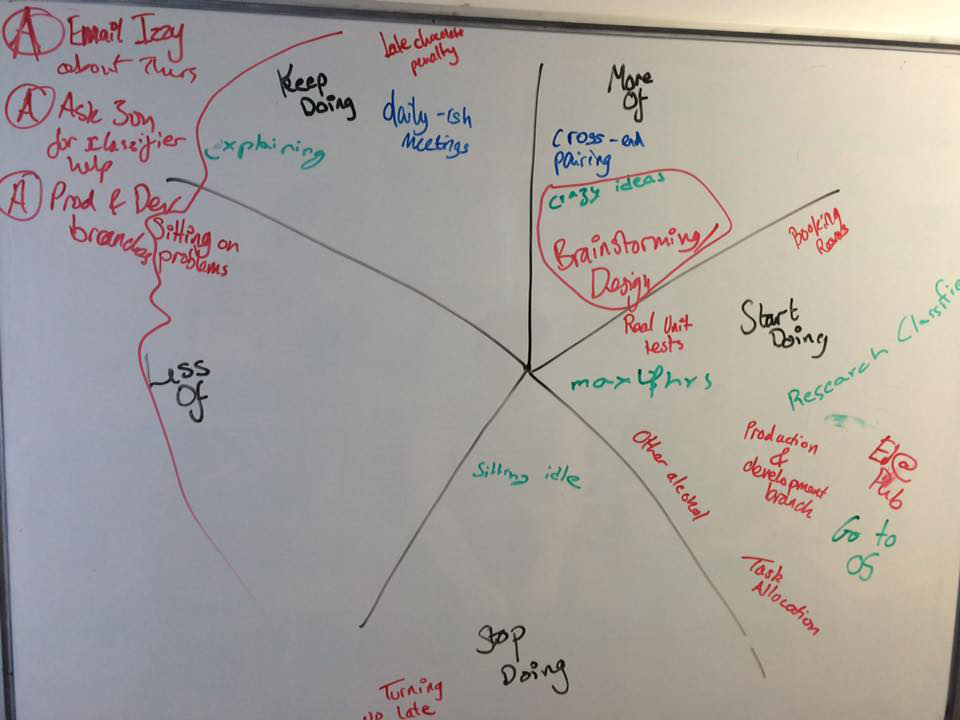
\includegraphics[width=0.8\textwidth]{figs/3/retro}
    \caption{One of our retrospectives}
    \label{fig:retro}
\end{figure}









\section{Project Management}
\subsection{Requirement Elicitation}
In order to create a Gantt chart, it had to determined which tasks were required to complete the project. Therefore in the first week a meeting was held with the project supervisor and industry customer to elicit key requirements from the software and their priorities. Thus emerged the initial task categories:

\begin{itemize}
\item General application
\item Interface
\item Grayscale vectorized images
\item Terrapattern conversion
\item Classifier
\item Feature Finder
\end{itemize}


\newpage
\subsection{MoSCoW}
Then, what these categories consisted of was determined by defining subtasks. In some cases various levels of a function were outlined. For example requirement C1.1 and C1.2 define a differing accuracy available. All of these requirements can be found in `Project Requirements' within appendix \ref{appendix:proj_reqs}. 

They have been prioritized via the MoSCoW method, where each task MUST/ SHOULD/ COULD/ WON'T be completed. This method is excellently intuitive for the customer and allowed for functionality discussions to flow smoothly.


\subsection{Gantt Chart}
Based on the nature of the project, there were two hard deadlines. On the 26$^{th}$ of October and 23$^{rd}$ of November, presentations had to be given on project progress. Therefore it was decided that this provided the team with three 4 week deliverables. Based on the companies we had experience with, 2 week sprints were the ideal balance of workload to work-based pressure.

When scheduling functionality, the ethos was `Minimum viable product'. The main idea being, if the project was dropped the day after a hard deadline, the Productizer would be a fully functioning tool. We also had to take into consideration the workload from other modules would increase over the semester. Therefore we scheduled 50\% of the workload to be complete in iteration one out of three, 30\% in iteration 2 and 20\% in iteration 3. This formed the gantt chart that can be seen in figure \ref{fig:gantt} below. 

\begin{figure}[H]
    \centering
    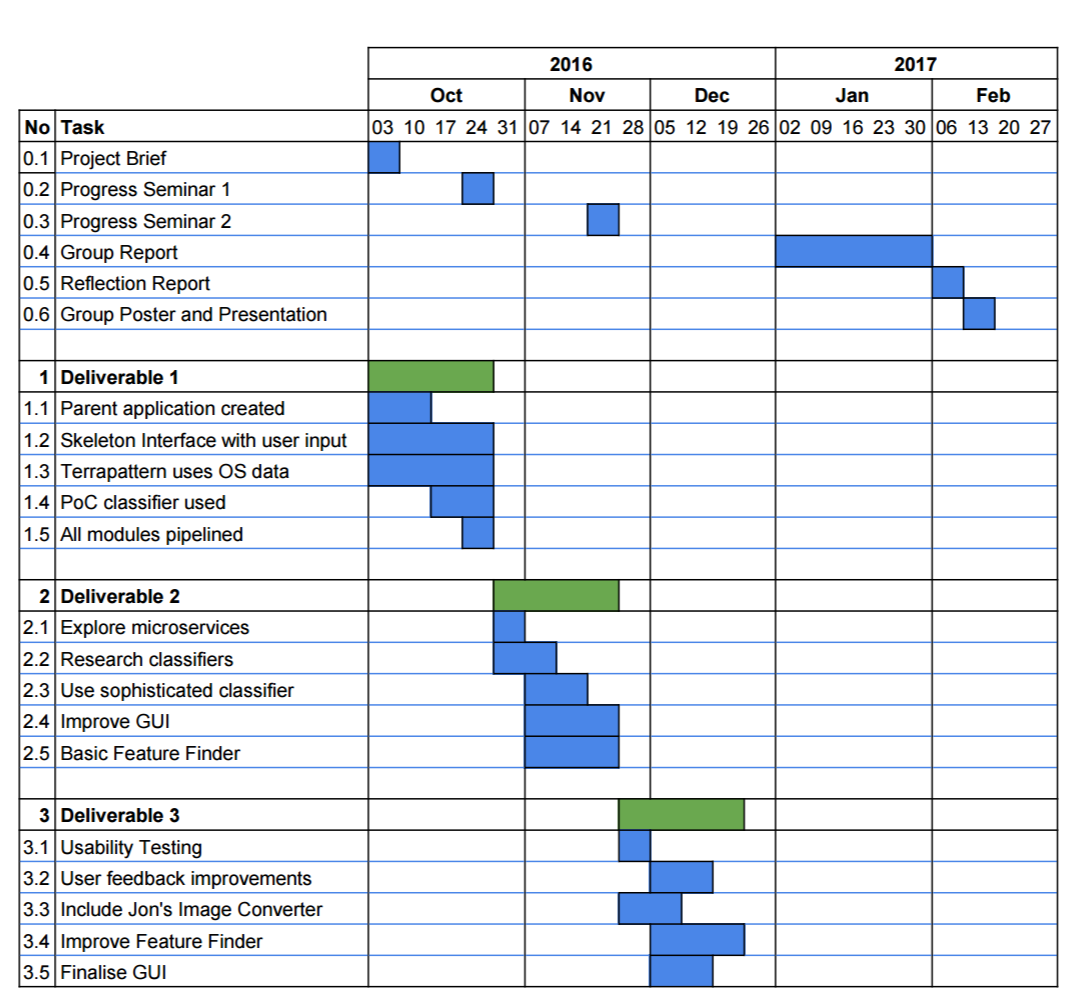
\includegraphics[width=1.1\textwidth]{figs/3/gantt}
    \caption{The Resulting Gantt Chart}
    \label{fig:gantt}
\end{figure}

\newpage

\subsection{Task Allocation}
Each task of a deliverable (from the Gantt chart) is comprised of a number of subtasks. To manage the completion of these tasks and subtasks, we kept sprint boards. 

\begin{figure}
    \centering
    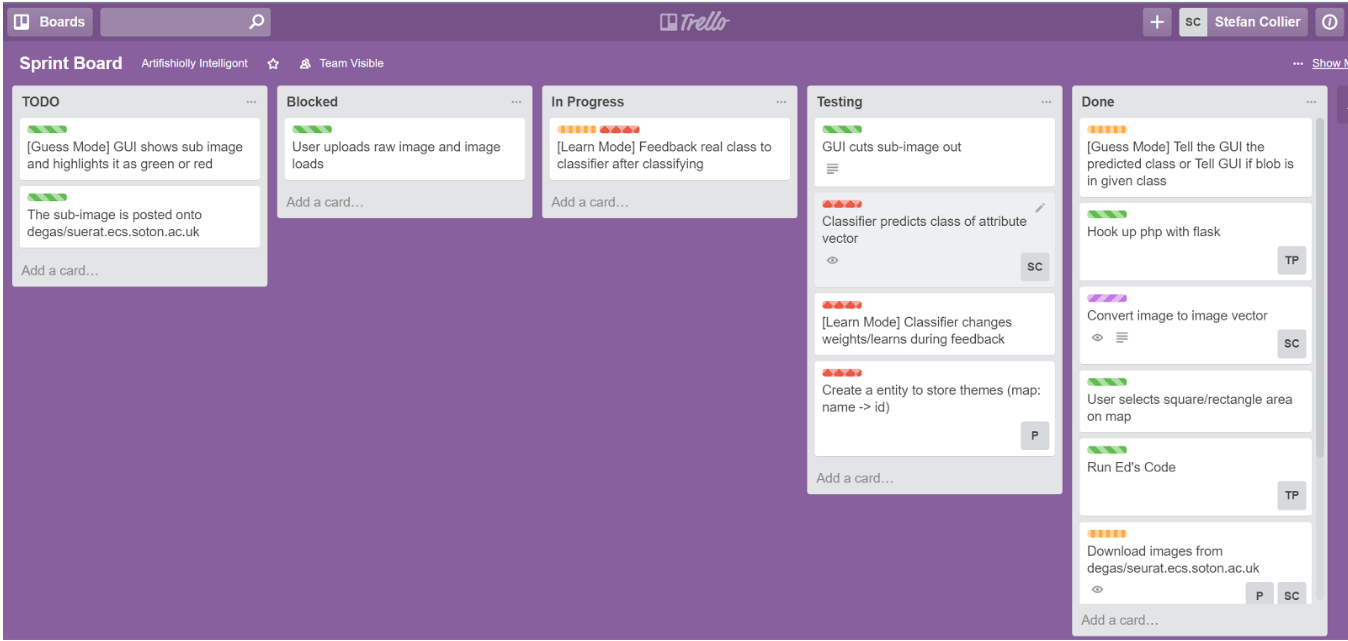
\includegraphics{figs/3/sprint_board}
    \caption{Sprint Board}
    \label{fig:sprint}
\end{figure}

Sprint boards are a fantastic method of scoping where the team is within the sprint. The consist of a number columns defining what stage of development a task is at. Tasks also belong to `Epics' which act as overriding themes (e.g. a GUI Epic). Self organising teams are a key aspect of agile development \citep{agile:manifesto}, as they encourage the best designs. The board enables developers to pick up tasks without concerns of conflict and by using Epics, they can easily guess if they have the domain knowledge for the task. 

\newpage
\subsection{Risk Analysis}
At the start of the project a list was compiled of risks and some contingency plans were completed. Note that impact and probability are out of 5 (where the larger the value implies a larger impact or chance of event). 


\begin{table}[H]
\centering
\label{my-label}
\begin{tabular}{@{}lcccl@{}}
\toprule
Risk                                                                                  & \begin{tabular}[c]{@{}c@{}}Impact\\ I\end{tabular} & \begin{tabular}[c]{@{}c@{}}Probability\\ P\end{tabular} & \begin{tabular}[c]{@{}c@{}}Rating\\ (P * I)\end{tabular} & Contingency                                                                                                         \\ \midrule
Ed going on holiday                                                                   & 4                                                  & 5                                                       & 20                                                       & \begin{tabular}[c]{@{}l@{}}- Deliverable-worth of work before \\ going\\ - Ed does handover\end{tabular}            \\ \midrule
\begin{tabular}[c]{@{}l@{}}Coursework from \\ other modules\end{tabular}              & 3                                                  & 5                                                       & 15                                                       & \begin{tabular}[c]{@{}l@{}}- Iteration 1 contained majority of\\  tickets(before courseworks released)\end{tabular} \\ \midrule
\begin{tabular}[c]{@{}l@{}}Team member\\  disappears/ is ill\end{tabular}             & 5                                                  & 1                                                       & 5                                                        & \begin{tabular}[c]{@{}l@{}}- Ensure no single specialists\\ - Share knowledge\end{tabular}                          \\ \midrule
\begin{tabular}[c]{@{}l@{}}Difficulty working \\ with Terrapattern\end{tabular}       & 3                                                  & 3                                                       & 9                                                        & \begin{tabular}[c]{@{}l@{}}- Use alternative image attribute\\  extractor\end{tabular}                              \\ \midrule
\begin{tabular}[c]{@{}l@{}}University source control \\ becomes unstable\end{tabular} & 5                                                  & 3                                                       & 15                                                       & - Use professional source control                                                                                   \\ \bottomrule
\end{tabular}
\caption{Key Considered Risk}

\end{table}

\section{Code}
\subsection{Pair Programming}
Pair Programing is the process of development where two people work together on one workstation to write code. By constantly swapping, both parties remain engaged \citep{pairing}. The main way to pair is the `Driver and Navigator' scenario. This is when two decide on a functionality to add and then the `Navigator' informs the `Driver' of instructions to perform; whilst checking the code for any bugs. 

During the first iteration, pair programming was used heavily. Due to the team's inexperience with the Python language this helped produce reliable code. When the experience party played the navigator, the driver learnt as they typed. When both parties were inexperienced then it helped prevent the driver from getting stuck as the navigator can determine what knowledge might be needed as the driver was writing. As the team became more experienced with Python, pairing occurred less frequently; being used for major or complex functions. 

This technique significantly reduced the need for peer reviewing work. It also ensured a transfer of knowledge in two ways. Participants learnt the language together, learning together was much faster than alone. This resulted in code quality increasing at a much faster rate and technical debt reducing each week. Participants also learn how other sections of the code functioned. This stopped the `reinvention of the wheel', auxiliary tools and helper functions were well known and widely used where necessary. 

\subsection{Distribution of Knowledge}
The team meetings (or `work days') of the first week of iteration 2, were strictly reserved for machine learning training. This was essential as only one team member had machine learning (ML) knowledge, research and development of ML-based systems was too much work for one person. The ML experience member taught the two server-side members the basics of machine learning, supervised, unsupervised learning techniques and briefly explained semi-supervised learning. 

This knowledge allowed the the entire server side team complete a group spike to determine the best classifier for the system. Not to mention being able to understand the code and intended purpose of it, which greatly helped testing. 


\subsection{Peer Review}
At the end of any significant task (that was completed individually), a developer would run through their work with another team member. Allowing for a the distribution of knowledge and bug checking that would have occurred if they pair programmed. This made certain of a good standard of code and reduced code redundancy whilst allowing both developers to make progress on separate tasks.

\subsection{Git}
In order to manage code version control, git and Github were used. All code was hosted as an `organisation' on github where our code could be privately managed. Each microservice had its own code repository to ensure modularity, thus avoiding merge issues during synchronous work. 

When doing day to development, code would be merged to the `dev' branch. The virtual machines would run off of the `prod' (i.e. production) branch. `dev' would be merged to `prod' once a fully tested and functioning feature had been completed. Therefore the services hosted on the virtual machines could be trusted during singular node testing. 






\section{Dev Tools and Tech}
In order to facilitate pair programming all server side code was written in the same IDE and likewise with the client side. Server side development was all handled via Pycharm and client-facing code was developed using Sublime Text 3. Uniformity was key amongst virtual machines as well, they all ran on Ubuntu 16, loaded with the same .bashrc and apache \& wgsi settings. However development occurred on both OSX, Ubuntu and Windows 10, all with varying screen dimensions. This allowed for various configurations to be tested for the client application.


\section{Division of Responsibilities}
The team consisted of 4 members. Each member had varied expertise and experience with concepts and tools. The team was collectively responsible for each all the code however table \ref{table:focus} shows how the team members distributed their time regarding the two sides of the project:

% Please add the following required packages to your document preamble:
% \usepackage{booktabs}
\begin{table}[H]
\centering
\caption{My caption}
\label{table:focus}
\begin{tabular}{@{}ll@{}}
\toprule
Team Member & Focus                                   \\ \midrule
Edward      & Client Facing                           \\
Prem        & Server Side                             \\
Stefan      & Server Side                             \\
Thomas      & Client Facing (33\%) \& Server Side (66\%) \\ \bottomrule
\end{tabular}
\end{table}

Even though each member shared the work of each service, by having a guardian for each service ensured there were final checks and tests. It also ensured that each team member had a particular expertise that helped when problems or questions were directed to the team: 

% Please add the following required packages to your document preamble:
% \usepackage{booktabs}
\begin{table}[H]
\centering
\begin{tabular}{@{}ll@{}}
\toprule
Team Member & Main Service          \\ \midrule
Edward      & Productizer (\&Grunt) \\
Prem        & Saturn                \\
Stefan      & Olivia                \\
Thomas      & Classifier            \\ \bottomrule
\end{tabular}
\caption{Key Responsibilities}
\end{table}


